\section{Аналитическая часть}

В данном разделе проводится анализ и выбор методов создания и рендера 
сложных твердотельных моделей.

\subsection{Анализ методов создания сложных твердотельных моделей}

Моделирование твёрдого тела --- это последовательный и 
непротиворечивый набор принципов математического и компьютерного 
моделирования трёхмерных твёрдых тел. 
На данном этапе рассмотрим 
существующие методы представления твёрдых тел.

\subsubsection{Клонирование примитивов}

Данный метод представления основан на понятии семейств объектов. 
Семейством называют группу объектов, отличающихся несколькими 
параметрами друг от друга. Например, с помощью операций поворота и 
масштабирования из исходного объекта можно получить семейство (рисуок \ref{fig:primitiveClone}).

\begin{figure}[h]
	\centering
	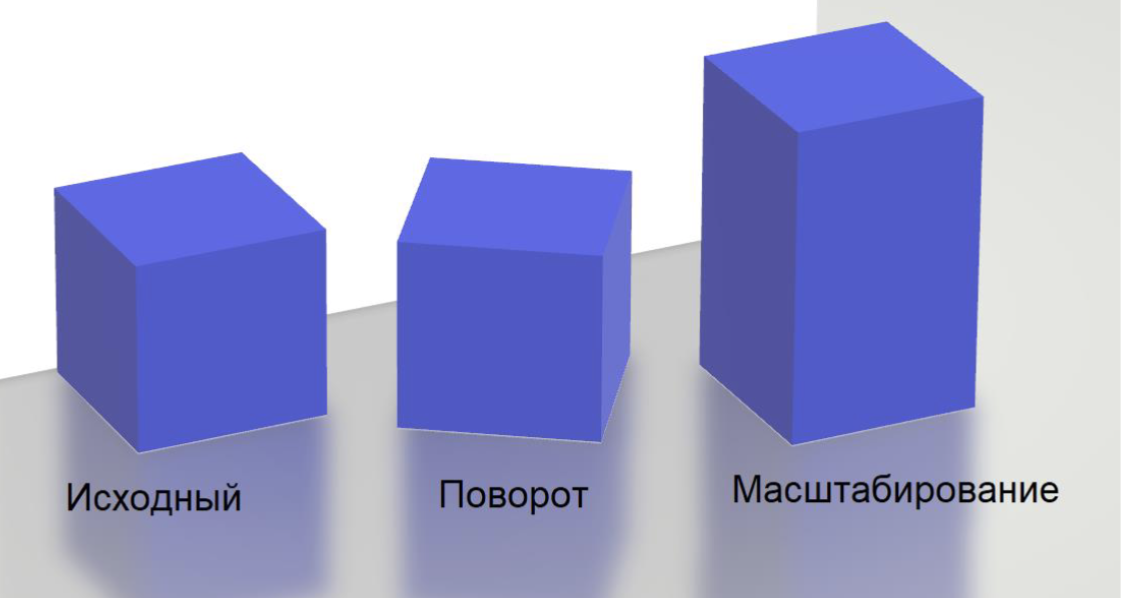
\includegraphics[width=\textwidth]{img/primitiveClone.png}
	\caption{Пример семейства объектов.}
	\label{fig:primitiveClone}
\end{figure}

При этом каждое семейство объектов называется общим примитивом, а 
отдельные объекты называются примитивными экземплярами. 
Так, семейство гаек является общим примитивом, а конкретная гайка, определённая набором характеристик, является примитивным экземпляром.
Особенностью данного методы является невозможность создать сложный 
объект сочетанием экземпляров. 
Рассмотрим плюсы и минусы. 

Минусом данного метода является сложность написания алгоритмов для вычисления свойств представленных тел --- отсутствие возможности написать общий алгоритм из-за уникальности примитивов ;

К плюсам можно отнести простоту реалзиации агоритма, если требуется представление только конкретного семейства моделей. 

Для решения поставленной задачи необходим метод, который позволит 
не зависеть от типа модели, её формы и параметров.  

Изучив данный метод, можно заключить, что он не подходит для решения 
поставленной задачи, так как возникает необходимость в подробном описании 
всех свойств определённого семейства, что будет проблематично осуществить 
для составных тел.

\subsubsection{Граничное представление}
В граничном представлении (\textit{англ.} Brep --- Boundary Representation) твердотельные модели представляются как совокупность 
двумерных границ, которые описывают трёхмерную модель. 
Твёрдое тело описывается как замкнутая пространственная область, ограниченная набором элементарных поверхностей (граней), имеющих образующие контуры (рёбра) на границе и признак внешней или внутренней стороны поверхности (см. 
рисунок \ref{fig:brep}). \newpage

\begin{figure}[h]
	\centering
	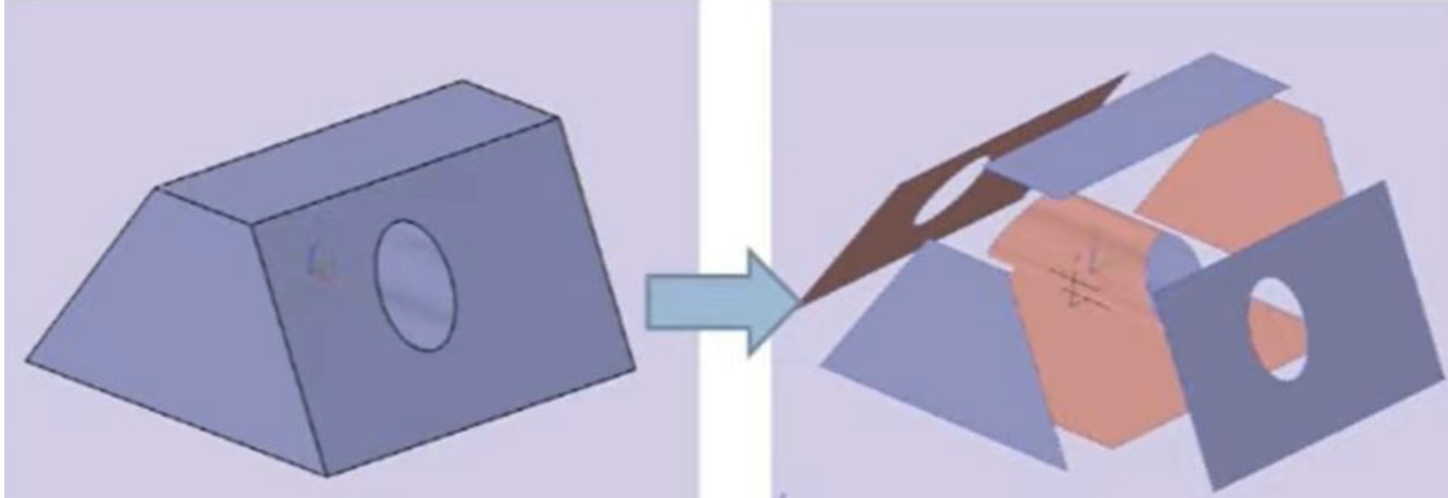
\includegraphics[width=\textwidth]{img/brep.png}
	\caption{Пример представления твёрдого тела как замкнутой 
		области и набором поверхностей.}
	\label{fig:brep}
\end{figure}

Такая схема проектирования крайне распространена в приложениях 
САПР, но, несмотря на это, она также имеет ряд недостатков, которые могут 
привести к проблемам визуализации результата.

Минусы:
\begin{itemize}[leftmargin=1.6\parindent]
	\item[---] большие затраты памяти;
	\item[---] проблемы получения описывающих формул в случае сложных объектов;
	\item[---] потребность в большой вычислительной мощности в момент рендера.
\end{itemize}

Плюсы:
\begin{itemize}[leftmargin=1.6\parindent]
	\item[---] метод походит не только для твёрдых тел с плоскими гранями, но и для 
	тел с криволинейными гранями или краями;
	\item[---] благодаря хранению информации о всех составляющих модели, метод 
	обеспечивает высокую точность;
	\item[---] метод позволяет эффективно хранить информацию о свойствах материалов получаемого тела.
\end{itemize}

Таким образом, данный метод не подходит для решения поставленной 
задачи, так как он требует значительное количество памяти для хранения 
необходимой информации, а также вычислительных мощностей в момент 
рендера.

\subsubsection{Нумерация пространственного заполнения (воксельный метод)} \label{sec:numeric}

Данный метод получил своё названия благодаря работе с 
пространственными ячейками (вокселями), который заполняют моделируемое 
тело.
Данные ячейки представляют собой кубы фиксированного размера и 
расположены в заданной пространственной сетке.
Полученный в результате 3D 
объект является совокупностью закрашенных вокселей (рис. \ref{fig:numeric}). 

\begin{figure}[h]
	\centering
	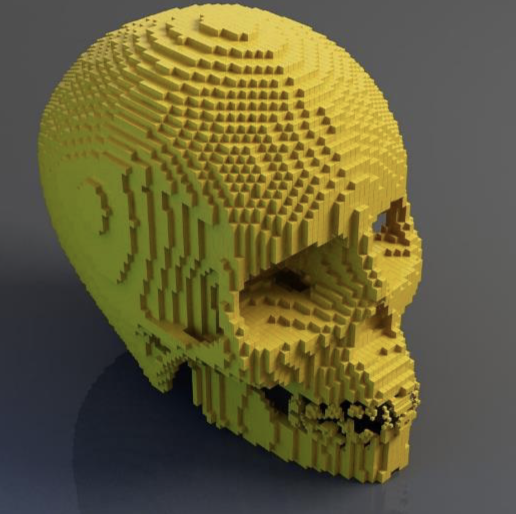
\includegraphics[width=110mm]{img/numeric.png}
	\caption{Пример изображения, полученного в результате 
		использования воксельного метода.}
	\label{fig:numeric}
\end{figure}

Каждая ячейка при этом должна быть представлена основной 
характеристикой --- например, координатами центра.
При сканировании 
обычно устанавливается определённый порядок обхода, а соответствующий 
упорядоченный набор координат называется пространственным массивом.

Такие пространственные массивы являются уникальными тведотельными 
представлениями, однако они слишком подробны для использования в качестве 
основного метода хранения модели.

Минусы:
\begin{itemize}[leftmargin=1.6\parindent]
	\item[---] большие затраты памяти;
	\item[---] каждая ячейка хранит информацию не только о своей координате, но и о цвете, плотности, оптических характеристиках и т. д.;
	\item[---] разрешение итогового изображения зависит от размера и формы вокселей.
\end{itemize}

Плюсы:
\begin{itemize}[leftmargin=1.6\parindent]
	\item[---] простота метода представления;
	\item[---] однозначность представления.
\end{itemize}

Простота и однозначность построения способствуют использованию 
данного метода при построении представлений, однако структурно 
использование кубических вокселей приводит к тому, что для рендера, например, сферы, будет необходимо проводить сглаживание краёв, что 
является дополнительной вычислительной нагрузкой

В нашем случае недостатком является и избыточная информация о 
каждой ячейке.
Таким образом, самостоятельное использование данного метода 
является неэффективным, однако в совокупности с другими методами можно 
использовать преимущества аппроксимации для повышения качества 
изображения тела.

\subsubsection{Октантное дерево}

Данная схема представления является улучшением воксельного метода. 
Строится октантное дерево, каждый узел которого соответствует некоторому 
кубу в трёхмерном пространстве, и для каждого куба определяется его 
принадлежность модели.
У каждого корня дерева есть 8 потомков, т.е. куб 
делится на 8 равных частей (рис.\ref{fig:octTree}).
\newpage

\begin{figure}[h]
	\centering
	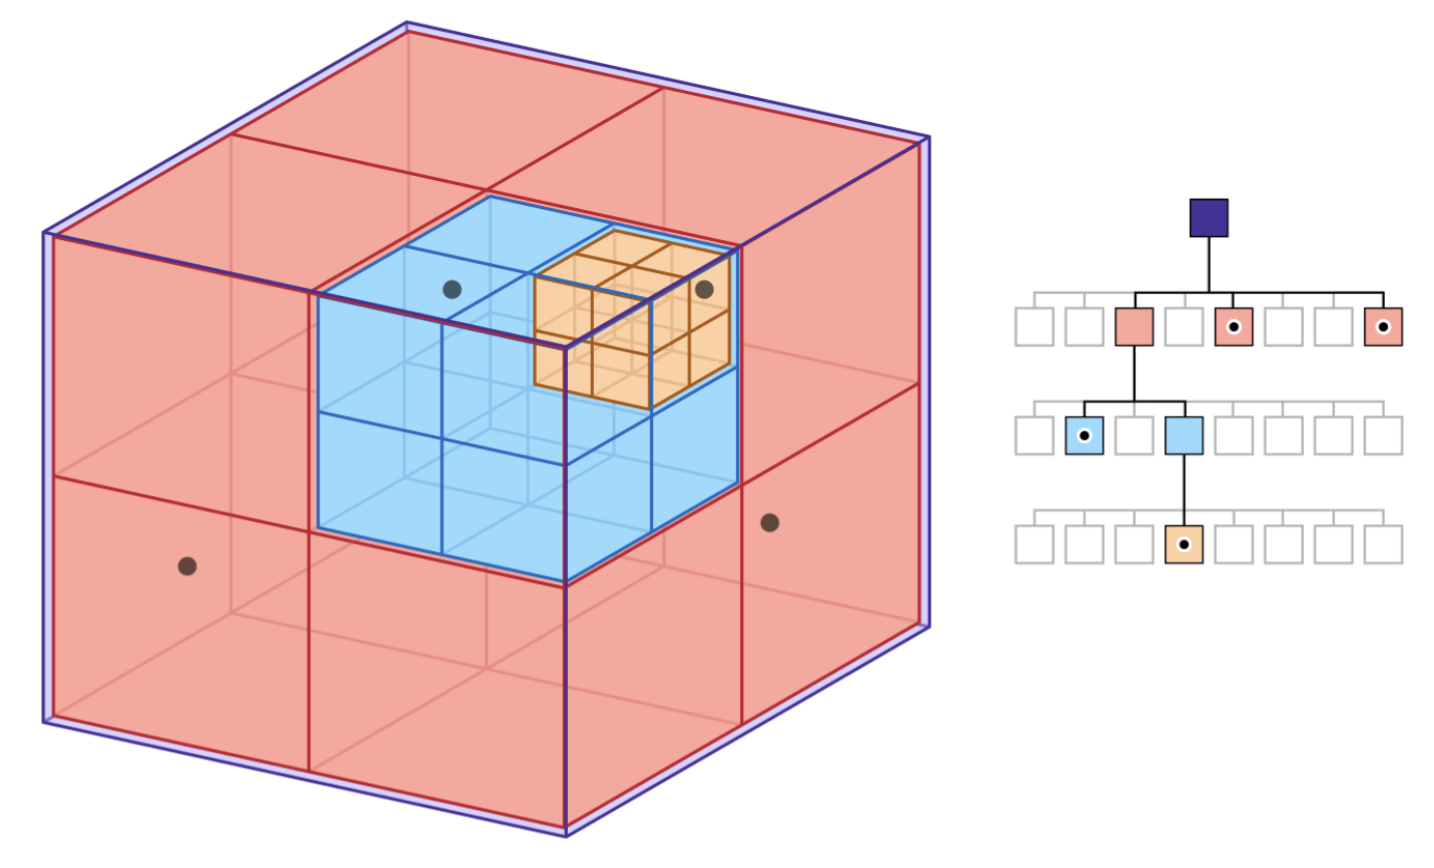
\includegraphics[width=\textwidth]{img/octTree.png}
	\caption{Разделение куба на 8 равных частей и получение 
		окнантного дерева.}
	\label{fig:octTree}
\end{figure}

Метод позволяет устранить недостаток метода \ref{sec:numeric}, 
связанного затратами памяти из-за хранения большого количества данных.
И хотя, сохраняя данные только об используемых частях модели, данный метод экономит память в сравнении с воксельным, по отношению к другим методам, 
памяти расходуется много.

Минусы:
\begin{itemize}[leftmargin=1.6\parindent]
	\item[---] деление примитива рёбрами кубов дерева может снижать 
	эффективность;
	\item[---] возможное выведение на экран невидимых объектов.
\end{itemize}

Плюсы:
\begin{itemize}[leftmargin=1.6\parindent]
	\item[---] простота метода представления;
	\item[---] однозначность представления.
\end{itemize}


\subsubsection{Выметание (Sweeping)}

Данный метод позволяет получить трёхмерную модель из двумерной 
посредством движения по заданной траектории (sweep), например, движения 
вокруг заданной оси или относительно грани (рис. \ref{fig:sweeping})

\begin{figure}[h]
	\centering
	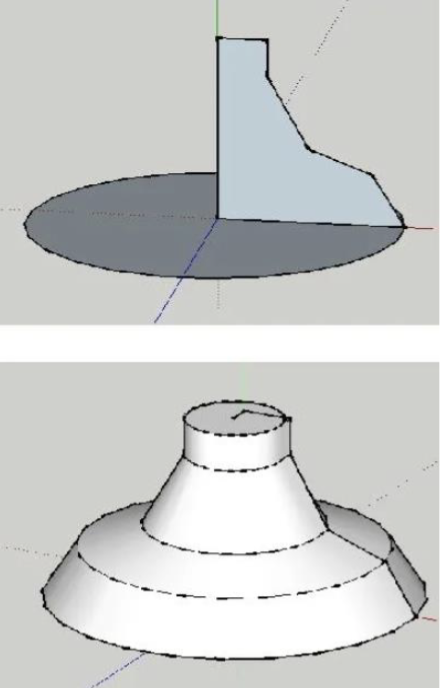
\includegraphics[width=80mm]{img/sweeping.png}
	\caption{Пример получения трёхмерного изображения посредством 
		вращения фигуры вокруг заданной оси.}
	\label{fig:sweeping}
\end{figure}

Недостатком данного метода является необходимость задавать траектории движения 2D объектов, что может быть проблематично для тел, имеющих сложную форму.

К преимуществам выметания можно отнести удобство определения простых форм через простые плоские фигуры, а также возможность использования метода для быстрого удаления материала внутри тела (рис. \ref{fig:deleting}). 
\newpage
\begin{figure}[h]
	\centering
	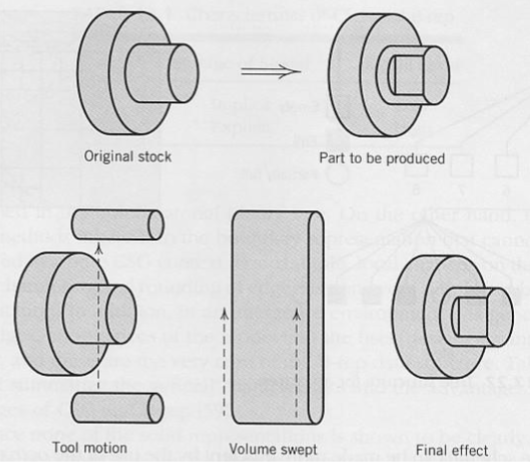
\includegraphics[width=80mm]{img/deleting.png}
	\caption{Пример удаления материала внутри тела посредством 
		алгоритма выметания.}
	\label{fig:deleting}
\end{figure}


\subsubsection{Конструктивная сплошная геометрия (CSG)}

Метод конструктивной сплошной геометрии основан на комбинировании 
примитивов посредством логических операций (объединения, пересечения, 
вычитания).
Любое составное тело может быть описано в виде традиционного 
уравнения из булевых функций, аргументами которого могут быть как 
примитивы, так и другие составные тела. 
Такое представление ещё называют 
деревом построений (рис. \ref{fig:csg}).

\begin{figure}[h]
	\centering
	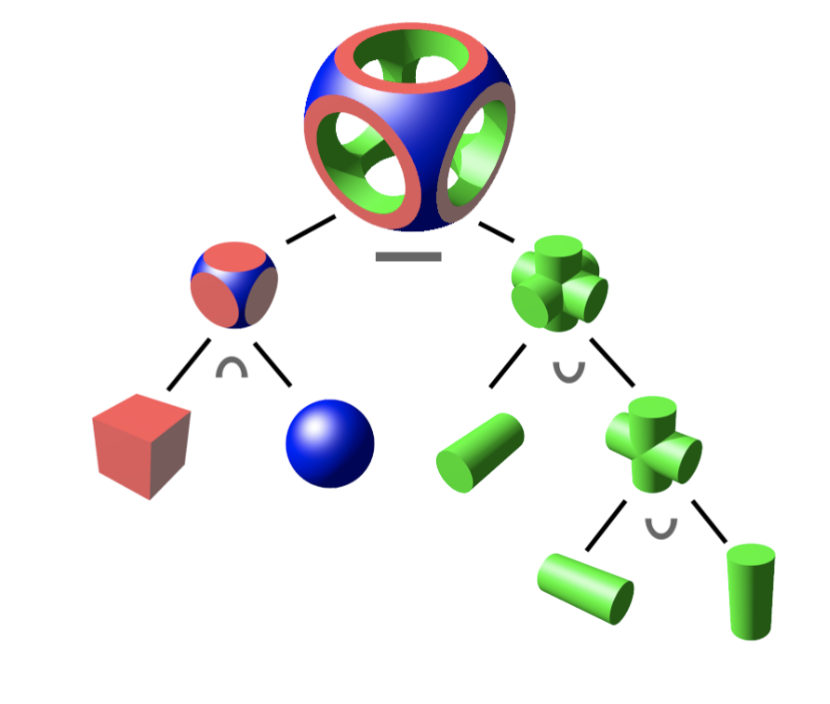
\includegraphics[width=120mm]{img/csg.png}
	\caption{Дерево построений при использовании CSG.}
	\label{fig:csg}
\end{figure}


\subsubs








Формула:

\begin{equation}
c^2 = a^2 + b^2
\end{equation}

Ссылаемся на рисунок \ref{fig:a1}. Информация из источника \cite{golang}.

\begin{figure}[hbtp]
	\centering
	
\includegraphics[width=\textwidth]{img/golang.png}
	\caption{Пример рисунка}
	\label{fig:a1}
\end{figure}

\begin{code}
	\captionof{listing}{Пример кода}
	\label{code:1}
	\inputminted
	[
	frame=single,
	framerule=0.5pt,
	framesep=20pt,
	fontsize=\small,
	tabsize=4,
	linenos,
	numbersep=5pt,
	xleftmargin=10pt,
	]
	{text}
	{code/main.go}
\end{code}

\pagebreak